\documentclass[../main]{subfiles}

\questiontrue
\solutiontrue

\begin{document}
    \ifquestion
    
    \section{Nill's Spaceship}
	
	As is well known, Nill das Graças was responsible for the illegal use of the Hubble Telescope in order to study the solar system with precision. To be able to use the telescope, Nill had to launch a spacecraft that would be positioned close to the target. Nill's spacecraft is a perfect spherical shell (where he is inside, obviously) with an inner radius \( r \) and an outer radius \( R \). The satellite's orbit is circular with a radius \( a \), and at a given moment, Nill is aligned with the center of the Earth and the center of the satellite at a distance \( x \) (\( x < r \)) from the center of the satellite, in the same direction and sense as the position vector of the satellite relative to the center of the Earth. Nill is in his own circular orbit. Find an algebraic expression for the time it takes for Nill to hit the wall of the satellite. Use any approximations you deem necessary, such as \( (1+x)^n \approx 1+nx \) and the approximation for the arccosine function: \( \arccos{(x)} \approx \sqrt{2-2x} \) for \( x \rightarrow 1^- \).
	
	\clearpage
    
    
    \fi
    
    \ifsolution
    
    	\section{Nill's Spaceship}
	
	Consider the following image as the representation of the described situation:
	
	\begin{figure}[htpb]
	    \centering
	    


\tikzset{every picture/.style={line width=0.75pt}} %set default line width to 0.75pt        

\begin{tikzpicture}[x=0.75pt,y=0.75pt,yscale=-1.2,xscale=1.2]
%uncomment if require: \path (0,542); %set diagram left start at 0, and has height of 542

%Shape: Circle [id:dp384256650616428] 
\draw   (350,122.51) .. controls (350,87.81) and (378.13,59.68) .. (412.83,59.68) .. controls (447.54,59.68) and (475.67,87.81) .. (475.67,122.51) .. controls (475.67,157.21) and (447.54,185.34) .. (412.83,185.34) .. controls (378.13,185.34) and (350,157.21) .. (350,122.51) -- cycle ;
%Straight Lines [id:da8273848420446885] 
\draw    (412.83,308.68) -- (412.83,124.51) ;
\draw [shift={(412.83,122.51)}, rotate = 90] [color={rgb, 255:red, 0; green, 0; blue, 0 }  ][line width=0.75]    (10.93,-3.29) .. controls (6.95,-1.4) and (3.31,-0.3) .. (0,0) .. controls (3.31,0.3) and (6.95,1.4) .. (10.93,3.29)   ;
\draw [shift={(412.83,308.68)}, rotate = 270] [color={rgb, 255:red, 0; green, 0; blue, 0 }  ][fill={rgb, 255:red, 0; green, 0; blue, 0 }  ][line width=0.75]      (0, 0) circle [x radius= 3.35, y radius= 3.35]   ;
%Straight Lines [id:da7228191470922871] 
\draw    (412.83,122.51) -- (412.83,80.01) ;
\draw [shift={(412.83,78.01)}, rotate = 90] [color={rgb, 255:red, 0; green, 0; blue, 0 }  ][line width=0.75]    (7.65,-2.3) .. controls (4.86,-0.97) and (2.31,-0.21) .. (0,0) .. controls (2.31,0.21) and (4.86,0.98) .. (7.65,2.3)   ;
\draw [shift={(412.83,122.51)}, rotate = 270] [color={rgb, 255:red, 0; green, 0; blue, 0 }  ][fill={rgb, 255:red, 0; green, 0; blue, 0 }  ][line width=0.75]      (0, 0) circle [x radius= 2.34, y radius= 2.34]   ;
%Straight Lines [id:da38974999198593596] 
\draw    (412.83,78.01) -- (412.83,122.51) ;
\draw [shift={(412.83,78.01)}, rotate = 90] [color={rgb, 255:red, 0; green, 0; blue, 0 }  ][fill={rgb, 255:red, 0; green, 0; blue, 0 }  ][line width=0.75]      (0, 0) circle [x radius= 2.34, y radius= 2.34]   ;

% Text Node
\draw (410.83,100.26) node [anchor=east] [inner sep=0.75pt]    {$x$};
% Text Node
\draw (410.83,215.59) node [anchor=east] [inner sep=0.75pt]    {$a$};
% Text Node
\draw (414.83,305.28) node [anchor=south west] [inner sep=0.75pt]    {$O$};
% Text Node
\draw (416.83,113.91) node [anchor=north west][inner sep=0.75pt]    {$S$};
% Text Node
\draw (416.17,66.74) node [anchor=north west][inner sep=0.75pt]    {$N$};


\end{tikzpicture}
	    \caption{Representation of the radial position of Nill in regard with his spaceship}
	    \label{fig:nillsspaceship1}
	\end{figure}

	Let "O" be the center of the Earth, "S" the center of the satellite, and "N" the position of Nill. Note that, by the shell theorem, there is no gravitational force between Nill and the satellite (since he is inside it), so the only force acting on Nill is the one from the Earth, which causes him to orbit in a circle of radius \( (a + x) \). Since the satellite orbits in a circle of radius \( a \), there is a difference between the orbital periods of Nill and the satellite. Equating the orbital periods:

\[
\frac{T_{S}^2}{a^3} = \frac{T_{N}^2}{(a + x)^3} = \frac{4\pi^2}{GM}
\]

\[
\therefore T_{N} = \sqrt{\frac{4\pi^2(a + x)^3}{GM}}
\]

\[
\therefore T_{S} = \sqrt{\frac{4\pi^2a^3}{GM}}
\]

After a time \( \Delta t \), the position vectors of S and N would have separated by an angle \( \alpha \), as shown in Figure \ref{fig:nill2}:


\begin{figure}[htpb]
	    \centering
	    

\tikzset{every picture/.style={line width=0.75pt}} %set default line width to 0.75pt        

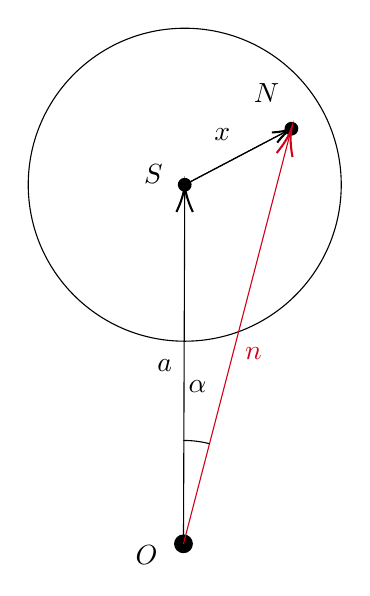
\begin{tikzpicture}[x=0.75pt,y=0.75pt,yscale=-1.2,xscale=1.2]
%uncomment if require: \path (0,542); %set diagram left start at 0, and has height of 542

%Shape: Circle [id:dp384256650616428] 
\draw   (350,122.51) .. controls (350,87.81) and (378.13,59.68) .. (412.83,59.68) .. controls (447.54,59.68) and (475.67,87.81) .. (475.67,122.51) .. controls (475.67,157.21) and (447.54,185.34) .. (412.83,185.34) .. controls (378.13,185.34) and (350,157.21) .. (350,122.51) -- cycle ;
%Straight Lines [id:da8273848420446885] 
\draw    (412.33,266.68) -- (412.83,124.51) ;
\draw [shift={(412.83,122.51)}, rotate = 90.2] [color={rgb, 255:red, 0; green, 0; blue, 0 }  ][line width=0.75]    (10.93,-3.29) .. controls (6.95,-1.4) and (3.31,-0.3) .. (0,0) .. controls (3.31,0.3) and (6.95,1.4) .. (10.93,3.29)   ;
\draw [shift={(412.33,266.68)}, rotate = 270.2] [color={rgb, 255:red, 0; green, 0; blue, 0 }  ][fill={rgb, 255:red, 0; green, 0; blue, 0 }  ][line width=0.75]      (0, 0) circle [x radius= 3.35, y radius= 3.35]   ;
%Straight Lines [id:da7228191470922871] 
\draw    (412.83,122.51) -- (453.9,100.94) ;
\draw [shift={(455.67,100.01)}, rotate = 152.29] [color={rgb, 255:red, 0; green, 0; blue, 0 }  ][line width=0.75]    (7.65,-2.3) .. controls (4.86,-0.97) and (2.31,-0.21) .. (0,0) .. controls (2.31,0.21) and (4.86,0.98) .. (7.65,2.3)   ;
\draw [shift={(412.83,122.51)}, rotate = 332.29] [color={rgb, 255:red, 0; green, 0; blue, 0 }  ][fill={rgb, 255:red, 0; green, 0; blue, 0 }  ][line width=0.75]      (0, 0) circle [x radius= 2.34, y radius= 2.34]   ;
%Straight Lines [id:da38974999198593596] 
\draw    (455.67,100.01) -- (412.83,122.51) ;
\draw [shift={(455.67,100.01)}, rotate = 152.29] [color={rgb, 255:red, 0; green, 0; blue, 0 }  ][fill={rgb, 255:red, 0; green, 0; blue, 0 }  ][line width=0.75]      (0, 0) circle [x radius= 2.34, y radius= 2.34]   ;
%Straight Lines [id:da7862253450322134] 
\draw [color={rgb, 255:red, 208; green, 2; blue, 27 }  ,draw opacity=1 ]   (412.33,266.68) -- (455.16,101.95) ;
\draw [shift={(455.67,100.01)}, rotate = 104.57] [color={rgb, 255:red, 208; green, 2; blue, 27 }  ,draw opacity=1 ][line width=0.75]    (10.93,-3.29) .. controls (6.95,-1.4) and (3.31,-0.3) .. (0,0) .. controls (3.31,0.3) and (6.95,1.4) .. (10.93,3.29)   ;
%Shape: Arc [id:dp9137849329227328] 
\draw  [draw opacity=0] (412.33,225.18) .. controls (412.33,225.18) and (412.33,225.18) .. (412.33,225.18) .. controls (415.93,225.18) and (419.41,225.63) .. (422.74,226.49) -- (412.33,266.68) -- cycle ; \draw   (412.33,225.18) .. controls (412.33,225.18) and (412.33,225.18) .. (412.33,225.18) .. controls (415.93,225.18) and (419.41,225.63) .. (422.74,226.49) ;  

% Text Node
\draw (432.17,102.26) node [anchor=east] [inner sep=0.75pt]    {$x$};
% Text Node
\draw (408.83,194.93) node [anchor=east] [inner sep=0.75pt]    {$a$};
% Text Node
\draw (392.03,276.08) node [anchor=south west] [inner sep=0.75pt]    {$O$};
% Text Node
\draw (395.5,113.24) node [anchor=north west][inner sep=0.75pt]    {$S$};
% Text Node
\draw (439.5,80.74) node [anchor=north west][inner sep=0.75pt]    {$N$};
% Text Node
\draw (436,186.74) node [anchor=north west][inner sep=0.75pt]  [color={rgb, 255:red, 208; green, 2; blue, 27 }  ,opacity=1 ]  {$n$};
% Text Node
\draw (413.33,200.14) node [anchor=north west][inner sep=0.75pt]    {$\alpha $};


\end{tikzpicture}
	    \caption{Variation of Nill's position in regards to time}
	    \label{fig:nill2}
	\end{figure}

	This angle can be calculated by the difference in the angular velocities of the objects (assuming they orbit in the same direction):

\[
\omega_{\text{rel}} = \omega_s - \omega_n = \frac{2\pi}{T_s} - \frac{2\pi}{T_n}
\]

\[
\omega_{\text{rel}} = \frac{2\pi\sqrt{GM}}{\sqrt{4\pi^2a^3}} - \frac{2\pi\sqrt{GM}}{\sqrt{4\pi^2(a+x)^3}} = \sqrt{\frac{GM}{a^3}} - \sqrt{\frac{GM}{(a+x)^3}}
\]

Assuming \( x \ll a \) and using the approximation \( (1 + y)^n \approx 1 + ny \), we have:

\[
\omega_{\text{rel}} = \sqrt{\frac{GM}{a^3}} - \sqrt{\frac{GM}{a^3(1 + x/a)^3}} = \sqrt{\frac{GM}{a^3}} - \sqrt{\frac{GM}{a^3}}(1 + x/a)^{-3/2}
\]

\[
\omega_{\text{rel}} \approx \sqrt{\frac{GM}{a^3}} - \sqrt{\frac{GM}{a^3}}\left(1 - \frac{3x}{2a}\right)
\]

\[
\therefore \omega_{\text{rel}} \approx \frac{3x}{2a}\sqrt{\frac{GM}{a^3}}
\]

Therefore, the angle \( \alpha \):

\[
\alpha = \omega_{\text{rel}} \Delta t = \sqrt{\frac{9x^2GM}{4a^5}} \Delta t
\]

Note that Nill will hit the edge of the satellite when the distance between N and S is equal to the inner radius of the spacecraft. Applying the law of cosines to triangle OSN to find SN:

\[
r^2 = a^2 + (a + x)^2 - 2a(a + x)\cos(\alpha)
\]

\[
\cos(\alpha) = \frac{a^2 + (a + x)^2 - r^2}{2a(a + x)}
\]

\[
\sqrt{\frac{9x^2GM}{4a^5}} \Delta t = \arccos{\left(\frac{a^2 + (a + x)^2 - r^2}{2a(a + x)}\right)}
\]

\[
\therefore \Delta t = \sqrt{\frac{4a^5}{9x^2GM}} \arccos{\left(\frac{a^2 + (a + x)^2 - r^2}{2a(a + x)}\right)}
\]

\[
\Delta t = \sqrt{\frac{4a^5}{9x^2GM}} \arccos{\left(1 + \frac{x^2 - r^2}{2a(a + x)}\right)}
\]

Since \( a \gg x \), we can approximate \( a + x \approx a \):

\[
\Delta t = \sqrt{\frac{4a^5}{9x^2GM}} \arccos{\left(1 - \frac{r^2 - x^2}{2a^2}\right)}
\]

Since \( r^2 - x^2 \ll a^2 \), we use the Taylor expansion of \( \arccos{x} \): \( \arccos{x} \approx \sqrt{2 - 2x} \) for \( x \rightarrow 1^- \):
	
    \[\Delta t = \sqrt{\frac{4a^5}{9x^2GM}}\frac{\sqrt{r^2-x^2}}{a}\]
    \[\therefore \Delta t = \frac{2a}{3x}\sqrt{\frac{a(r^2-x^2)}{GM}}\]
	
	\clearpage
    
    
    \fi
\end{document}
